\nextpage
\section{Опыт А. Четыре сканера}
Какой сканер быстрее на учебном корпусе и сохранится ли его преимущество при замене текста? В первом опыте время включает весь путь от чтения очередного байта до выдачи и учёта лексемы. Каждый столбец таблицы~\ref{tab:a} получен из одной и той же серии раундов.

\begin{center}
\captionof{table}{Время четырёх сканеров в нс/байт. В каждой ячейке сверху дана медиана, снизу~--- $[Q_1;Q_3]$. $N$ измеряется в байтах, $K$~--- число лексем без EOF.}\label{tab:a}
\setlength{\tabcolsep}{2pt}
\fontsize{9.1}{10.5}\selectfont
\begin{tabular*}{\linewidth}{@{\extracolsep{\fill}}lrrcccc@{}}
\toprule Вход & $N$ & $K$ & flex & re2c & table & branch\\ \midrule
\rowsA
\bottomrule
\end{tabular*}
\end{center}
На корпусе первым оказался re2c. Даже его верхний квартиль (2,561~нс/байт) ниже нижнего квартиля ближайшего варианта branch (3,386~нс/байт). На двухбайтовых именах и числах, а также на всех трёх размерах смешанного текста наименьшее время показала таблица.

\nextpage
\section*{Когда меняется самый быстрый сканер}
При фиксированном объёме одна переменная особенно заметно меняет результат: сколько байтов успевает прочитать сканер до очередной выдачи лексемы. На рис.~\ref{fig:length} для каждой длины взяты данные из двух строк таблицы~\ref{tab:a}, одной с буквами и одной с цифрами.

\begin{center}
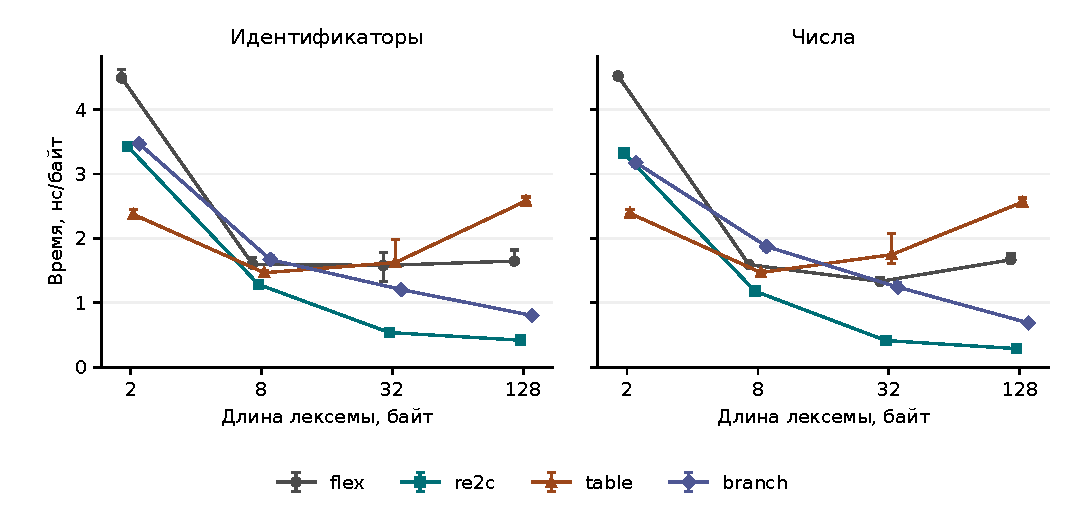
\includegraphics[width=\linewidth]{figures/length.pdf}
\captionof{figure}{Медиана времени полного прохода на байт при объёме $2^{20}$ байт. Маркеры различают четыре реализации, вертикальные отрезки показывают $[Q_1;Q_3]$. Горизонтальная ось логарифмическая по основанию 4, значения подписаны в байтах. Маркеры немного разведены по горизонтали для чтения интервалов.}\label{fig:length}
\end{center}

\subhead{Короткое слово и длинное слово}
При длине~2 наименьшая медиана у table в обеих сериях, а начиная с проверенной длины~8~--- у re2c. У последнего на числах она падает с 3,322 до 0,288~нс/байт. На идентификаторах той же длины~--- с 3,429 до 0,419. При этом $K$ уменьшается с 349\,525 до 8\,128. Время учёта одной выдачи распределяется на большее число байтов. Одного этого объяснения недостаточно: у table время на байт при переходе с 32 до 128 букв, наоборот, возрастает.

\subhead{Повторение одного и того же оператора}
На младшем, среднем и старшем объёмах у table получено 2,161, 2,159 и 2,197~нс/байт. Их межквартильные интервалы перекрываются. Объём самого большого файла в 256 раз больше первого. Полное время прохода возрастает примерно с 0,133 до 34,56~мс. Для этой периодической смеси переход к большому файлу мало изменил расходы на байт. Три размера не определяют закон роста для произвольного текста.

\subhead{Пограничные случаи}
По минимуму медианы re2c оказался первым на 11 входах, table~--- на 10. На \code{abcde2} медианы этих программ отличаются на 0,004~нс/байт. На длинных комментариях у re2c и branch получены 1,388 и 1,397~нс/байт. На первом входе table опередил re2c в 10 раундах из 16, на втором re2c опередил branch в 9 из 16. У каждой пары разница медиан мала на фоне разброса.
